%
\documentclass[12pt]{article}

% The usual packages
\usepackage{fullpage}
\usepackage{breakcites}
\usepackage{setspace}
\usepackage{endnotes}
%\usepackage{float} % can't use with floatrow
\usepackage{amsmath}
\usepackage{amsfonts}
\usepackage{amssymb}
\usepackage{rotating}
\usepackage{longtable}
\usepackage{microtype}
\usepackage{graphicx}
\usepackage{hyperref}
%\usepackage[usenames,dvipsnames]{color}
\usepackage{url}
\usepackage{natbib}
\usepackage{framed} 
\usepackage{epigraph}
\usepackage{lipsum}
\usepackage{enumerate}
%\usepackage{dcolumn}
%\restylefloat{table}
\bibpunct{(}{)}{;}{a}{}{,}

% Set paragraph spacing the way I like
\parskip=0pt
\parindent=20pt

%\usepackage{helvet}
\usepackage[labelfont={bf}, margin=0cm, font=small, skip=0pt]{caption}


% Define mathematical results
\newtheorem{lemma}{Lemma}
\newtheorem{proposition}{Proposition}
\newtheorem{theorem}{Theorem}
\newtheorem{claim}{Claim}
\newenvironment{proof}[1][Proof]{\begin{trivlist}
\item[\hskip \labelsep {\bfseries #1}]}{\end{trivlist}}
\newenvironment{definition}[1][Definition]{\begin{trivlist}
\item[\hskip \labelsep {\bfseries #1}]}{\end{trivlist}}
\newenvironment{example}[1][Example]{\begin{trivlist}
\item[\hskip \labelsep {\bfseries #1}]}{\end{trivlist}}
\newenvironment{remark}[1][Remark]{\begin{trivlist}
\item[\hskip \labelsep {\bfseries #1}]}{\end{trivlist}}
\DeclareMathOperator*{\argmin}{arg\,min}
\DeclareMathOperator{\med}{med}


% Set up fonts the way I like
%\usepackage{tgpagella}
%\usepackage[T1]{fontenc}
%\usepackage[bitstream-charter]{mathdesign}

%% Baskervald
%\usepackage[lf]{Baskervaldx} % lining figures
%\usepackage[bigdelims,vvarbb]{newtxmath} % math italic letters from Nimbus Roman
%\usepackage[cal=boondoxo]{mathalfa} % mathcal from STIX, unslanted a bit
%\renewcommand*\oldstylenums[1]{\textosf{#1}}

%\usepackage[T1]{fontenc}
%\usepackage{newtxtext,newtxmath}

% A special command to create line break in table cells
\newcommand{\specialcell}[2][c]{%
 \begin{tabular}[#1]{@{}c@{}}#2\end{tabular}}


%% Set up lists the way I like
% Redefine the first level
\renewcommand{\theenumi}{\arabic{enumi}.}
\renewcommand{\labelenumi}{\theenumi}
% Redefine the second level
\renewcommand{\theenumii}{\alph{enumii}.}
\renewcommand{\labelenumii}{\theenumii}
% Redefine the third level
\renewcommand{\theenumiii}{\roman{enumiii}.}
\renewcommand{\labelenumiii}{\theenumiii}
% Redefine the fourth level
\renewcommand{\theenumiv}{\Alph{enumiv}.}
\renewcommand{\labelenumiv}{\theenumiv}
% Eliminate spacing around lists
\usepackage{enumitem}
\setlist{nolistsep}

% Create footnote command so that my name
% has an asterisk rather than a one.
\long\def\symbolfootnote[#1]#2{\begingroup%
\def\thefootnote{\fnsymbol{footnote}}\footnote[#1]{#2}\endgroup}

% Create the colors I want
\usepackage{color}
\definecolor{darkred}{RGB}{100,0,0}

\hypersetup{
pdftitle={When BLUE Is Not Best}, % title
pdfauthor={Dan K. Baissa and Carlisle Rainey}, % author
pdfkeywords={robust linear regression} {outliers} {leverage}
pdfnewwindow=true, % links in new window
colorlinks=true, % false: boxed links; true: colored links
linkcolor=black, % color of internal links
citecolor=black, % color of links to bibliography
filecolor=black, % color of file links
urlcolor=blue % color of external links
}

% section headers
%\usepackage[scaled]{helvet}
%\renewcommand\familydefault{\sfdefault} 
%\usepackage[T1]{fontenc}
%\usepackage{titlesec}
%\titleformat{\section}
%  {\normalfont\sffamily\Large\bfseries}
%  {\thesection}{1em}{}
%\titleformat{\subsection}
%  {\normalfont\sffamily\large\bfseries}
%  {\thesection}{1em}{}
%  \titleformat{\subsubsection}
%  {\normalfont\sffamily\bfseries}
%  {\thesection}{1em}{}

% enable comments in pdf
\newcommand{\dtk}[1]{\textcolor{blue}{#1}}
\newcommand{\ctk}[1]{\textcolor{red}{#1}}


\begin{document}

\begin{center}
{\LARGE \textbf{When BLUE Is Not Best}}\\\vspace{2mm}
{ \textbf{Non-Normal Errors and the Linear Model}\symbolfootnote[1]{We thank Bill Clark and Matt Golder for making their data available to us. The analyses presented here were conducted with \texttt{R} 3.2.2. All data and computer code necessary for replication are available at \href{https://github.com/carlislerainey/heavy-tails}{
github.com/carlislerainey/heavy-tails}.}}\\\vspace{2mm}


\vspace{10mm}

Daniel K. Baissa\symbolfootnote[2]{Daniel K. Baissa is a Ph.D. student in the Department of Government, Harvard University, 1737 Cambridge St., Cambridge, MA, 02138 (\href{mailto:dbaissa@g.harvard.edu}{dbaissa@g.harvard.edu}).}

\vspace{3mm}

Carlisle Rainey\symbolfootnote[3]{Carlisle Rainey is Associate Professor of Political Science, Florida State University, Room 531B Bellamy Building, 113 Collegiate Loop, Tallahassee, FL, 32306 (\href{mailto:crainey@fsu.edu}{crainey@fsu.edu}).}
\end{center}

\vspace{10mm}

% Abstract
{\centerline{\textbf{Abstract}}}
\begin{quote}\noindent
Researchers in political science often estimate linear models of continuous outcomes using least squares. 
While it is well-known that least-squares estimates are sensitive to single, unusual data points, this knowledge has not led to careful practices when using least-squares estimators. 
Using statistical theory, Monte Carlo simulations, and an applied example, we highlight the importance of using more robust estimators along with variable transformations.
We also discuss several approaches to detect, summarize, and communicate the influence of particular data points. 
 \end{quote}

% Add quote to first page
% \epigraph{}

%\begin{center}
%Manuscript word count: 
%\end{center}

% Remove page number from first page
\thispagestyle{empty}

% Start main text
\newpage
\doublespace

\section*{Introduction}

Linear models of the form $y_i = X_i\beta + \epsilon_i$ estimated with least squares remain one of the most common statistical tools in political science research \citep{KruegerLewisBeck2008}. 
Yet some confusion still exists about the conditions under which least squares serves as a good estimator of the linear model. 
After assuming that the model $y_i = X_i\beta + \epsilon_i$ is correct and that the matrix $X$ is full rank, we need to make further assumptions about the errors $\epsilon_i$ to obtain desirable properties for the least-squares estimator. We might use some of the following assumptions:
\begin{enumerate}[label= A\arabic*:]
  \item Errors have mean equal to zero.
  \item Errors have a constant, finite variance.
  \item Errors are independent.
  \item Errors follow a normal distribution.
\end{enumerate}
By assuming only A1, we obtain an unbiased, consistent estimator (e.g., \citealt{Wooldridge2013}, p. 810 and pp. 385, 815--816). 
However, by assuming A1, A2, A3, and A4, we obtain the best unbiased estimator (BUE), which has the smallest possible variance among the class of unbiased estimators (e.g., \citealt{Wooldridge2013}, pp. 809--815).

However, political scientists tend to focus on a different property of least squares. By the Gauss-Markov theorem, we can remove A4---the assumption of normal errors---and still obtain the best \textit{linear} unbiased estimator (BLUE), which has the smallest possible variance among the class of unbiased, \textit{linear} estimators (e.g., \citealt{Wooldridge2013}, pp. 809--812). 
Researchers have primarily justified least squares using the Gauss-Markov theorem because it seems to impart desirable small-sample properties without the overly restrictive assumption of normal errors.
For example, \cite{BerryFeldman1985} write: 
\begin{quote}
[The assumption of normally distributed errors] is necessary \textit{only} for tests of significance; its violation will have no effect on the estimation of the parameters of the regression model. It is quite fortunate that normality is not required for estimation, because it is often very difficult to defend this assumption in practice.\footnote{Similarly, \citet[p. 101]{Wooldridge2013} writes that the Gauss-Markov theorem ``justifies the use of the OLS method rather than using a variety of competing estimators.''}
\end{quote}

However, notice that a tradeoff occurs when relaxing the assumption of normal errors. 
To relax the assumption of normal errors (and keep desirable small sample properties), we must restrict ourselves to linear estimators. 
This raises a critical, but often overlooked question: Under what conditions can a researcher safely restrict herself to linear estimators? 
We argue that a restriction to linear estimators makes sense only when the errors follow a normal distribution. 
If the errors do not follow a normal distribution, then least-squares is still a best \textit{linear} unbiased estimator, but other, non-linear estimators may be more more efficient.
Our claim is that the restriction to linear estimators is artificial and can only be justified by assuming normal errors---an assumption that \cite{BerryFeldman1985} note is very difficult to defend in practice.

The Gauss-Markov theorem has convinced researchers in political science that as long as A1, A2, and A3---the Gauss-Markov assumptions---are met, the distribution of the errors is unimportant. 
But the distribution of the errors is crucial to a linear regression analysis.
Deviations from normality, especially large deviations commonly found in regression models in political science, can devastate the performance of least squares compared to alternative estimators. Perhaps even more importantly, regression residuals offer detailed substantive information that researchers often ignore.

In our paper, we emphasize the importance of errors and residuals from a statistical and substantive perspective. We adopt and defend a skeptical perspective toward least squares in favor of more robust estimators. We proceed as follows: we (1) clarify the crucial distinction between a linear \textit{model} and a linear \textit{estimator}, (2) explain that the BLUE estimator is not the best estimator unless the errors are normally distributed, (3) highlight powerful, robust alternatives to least-squares estimators that are unbiased and more efficient for a wide range of substantively plausible error distributions, (4) provide concrete, practical advice to substantive researchers using linear models, and (5) provide a compelling example that illustrates the importance of robust estimators.

\section*{Is a BLUE Estimator the Best Estimator?}

The linear model can be written as $y = X\beta + \epsilon$.\footnote{As usual, $y$ is an outcome variable of interest (usually roughly continuous), $X$ is a $n \times (k + 1)$ matrix containing a single column of ones and $k$ columns holding $k$ explanatory variables, $\beta$ is a $(k + 1) \times 1$ matrix of model coefficients, and $\epsilon$ is an $n \times 1$ matrix of errors. As usual, the statistical properties of these estimators depend on this model being correct and a full rank $X$.} 
Researchers in political science commonly estimate this model with least squares by minimizing the sum of the squared residuals, such that $\hat{\beta}^{ls} = \argmin_b S(b)$, where $S(b) = \sum_{i = 1}^n(y_i - X_ib)^2$. 
If we assume that the errors $\epsilon$ follow independent and identical normal distributions with mean zero and unknown variance, which we refer to as a ``normal-linear model,'' then the least squares estimator is the best (i.e., minimum variance) unbiased estimator (BUE) (\citealt[pp. 334--342]{CasellaBerger2002}, and \citealt[807--815]{Wooldridge2013}).
This is a powerful result. 
Under the assumption of normally distributed errors, least squares is the most efficient unbiased estimator.

\subsection*{The Unreasonable Restriction to Linear Estimators}

If we relax the assumption of normality and simply require that the errors have mean zero and constant variance, then the Gauss-Markov Theorem guarantees that the least-squares estimator is the best \textit{linear} unbiased estimator. 
While this result is often emphasized, it should provide little comfort to researchers because there is little statistical or substantive reason to restrict themselves to \textit{linear} estimators.

At first glance, one might take the linearity restriction in the Gauss-Markov theorem to refer to the structure of the model (i.e., ``linear in the parameters''). 
Indeed, this is the sense in which we use ``linear'' in the phrase ``linear model.'' 
However, the ``linear'' restriction in the Gauss-Markov Theorem refers to a different concept---a linear \textit{estimator}, which is a technical condition that has little connection to the substance of the problem.
Linearity of the \textit{estimator} requires that the estimates be a linear function of the outcome variable, so that $\hat{\beta}_j = \lambda_1 y_1 + \lambda_2 y_2 + ... + \lambda_n y_n$, where the weights $\lambda_i$ are allowed to depend on $X$, but not on $y$. 
In other words, the Gauss-Markov theorem assumes a linear \textit{model} of the form $E(y | X) = X\beta$, but it also restricts researchers to linear \textit{estimators} of the form $\hat{\beta}_j = \lambda_1 y_1 + \lambda_2 y_2 + ... + \lambda_n y_n$.\footnote{Simple algebra shows that the least-squares criterion produces a linear estimator. 
First, recall that we wish to minimize $S(b) = \sum_{i = 1}^n(y_i - X_ib)^2$ with respect to $b$. 
To minimize $S(b)$, set $\dfrac{\partial S(\hat{\beta}^{ls})}{\partial \hat{\beta}^{ls}} = 0$ and solve for the vector $\hat{\beta}^{ls}$. 
$\dfrac{\partial S(\hat{\beta}^{ls})}{\partial \hat{\beta}^{ls}} = \sum_{i = 1}^n 2(y_i - X_i\hat{\beta}^{ls})(-X_i) = 0$ implies that $\sum_{i = 1}^n X_i(y_i - X_i\hat{\beta}^{ls}) = 0$. 
This is a system of $k+1$ \textit{linear} equations $\sum_{i = 1}^n X_{ij}(y_i - X_i\hat{\beta}^{ls})$ for $j = \{0, 1, 2,..., k\}$. 
Of course, the matrix form $X'(y - X\hat{\beta}^{ls}) = 0 \Rightarrow (X'X)\hat{\beta}^{ls} = X'y \Rightarrow \hat{\beta}^{ls} = (X'X)^{-1}X'y$ is much more common. 
In matrix form, linearity of the estimator requires that $\hat{\beta} = My$, where $M$ depends on the matrix $X$. 
We can clearly see that the least squares estimator $\hat{\beta}^{ls} = (X'X)^{-1}X'y$ has the form $My$.}

However, restricting ourselves to linear estimators is neither necessary nor productive. 
We are not arguing against linear models (i.e., linear in the parameters), such as 
\begin{align}
y_i &= \beta_0 + \beta_1\log(x_i) + \epsilon_i\text{,}\\
y_i &= \beta_0 + \beta_1x_i + \beta_2x_i^2 + \epsilon_i\text{, or}\\ 
y_i &= \beta_0 + \beta_1x_i + \beta_2z_i + \beta_3x_iz_i + \epsilon_i\textit{.}
\end{align}
Indeed, we encourage the use of these models. This collection of linear models illustrates that the linear model can represent a wide range of theoretically-relevant relationships, especially when it includes explanatory variables non-linearly. 
Crucially, though, \textit{there is no statistical reason to restrict ourselves to linear \textit{estimators} for these linear models}, except for mathematical convenience and computational ease.
The only substantive reason to restrict ourselves to linear estimators is if we are willing to assume that we have normally distributed errors. 
Under the assumption of normal errors, linearity is a reasonable restriction---indeed, the linear estimator is BUE when the errors are normal.
Crucially, restriction to linearity does not get us away from the assumption of normality because BLUE estimators are BUE estimators only under the assumption of normal errors.
If the errors are not normally distributed, then a researcher can easily better the BLUE estimator.

%But we might also make a substantive argument \textit{against} linear estimators (i.e., weighting all observations equally). 
%We suggest two potentially desirable properties of estimators. 
%First, we might prefer estimators that provide an excellent fit to \textit{most} of the data rather rather than a mediocre fit to \textit{all} the data. 
%Secondly, we might prefer an estimate that treats unusual data equally---as inconsistent with the model.
%Neither of these behaviors is possible with linear estimators.
%
%For example, consider the estimates shown in the left panel of Figure~\ref{fig:best-fit-illustration}. 
%Which of the two estimates, A or B, best summarizes the relationship between the explanatory and outcome variable? 
%Estimate A fits all the data reasonably well, but estimate B provides an excellent summary for most of the data. 
%Which is preferred? 
%At least in some cases, we might prefer estimate B because we wish to discount the three unusual cases as inconsistent with the model (perhaps these cases are elections marred with scandals, etc.).
%
%\begin{figure}[h!]
%\begin{center}
%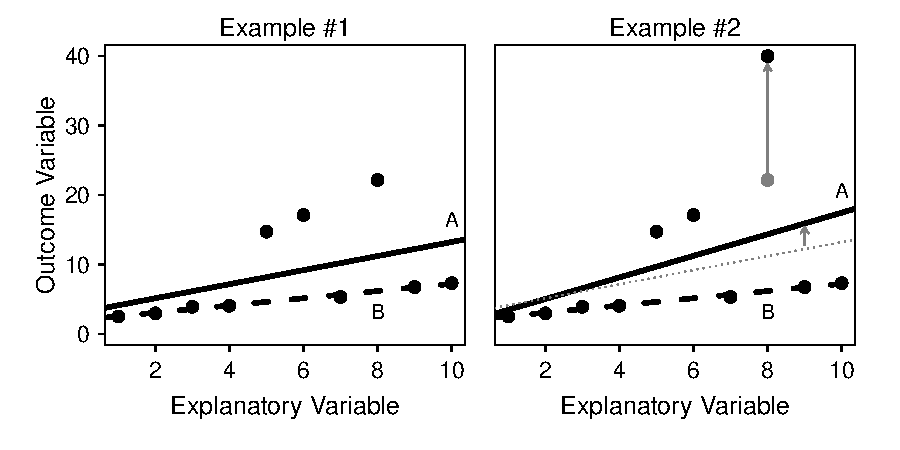
\includegraphics[scale = .7]{figs/best-fit-illustration.pdf}
%\caption{This figure shows to hypothetical examples that illustrate two potentially desirable properties of estimators.
%The left panel illustrates that one estimator (A) might provide an excellent fit to most of the data while another estimator (B) might provide a mediocre fit to all the data. 
%The right panel illustrates that one estimator (A) might ignore changes among the unusual cases while anther estimator (B) might be quite responsive.}\label{fig:best-fit-illustration}
%\end{center}
%\end{figure}
%
%Secondly, we might prefer an estimator that gives zero weight to cases that fall outside the explanatory power of the model.
%These cases seem somehow different and we might prefer that these unusual data to not degrade the excellent fit for the majority of the data. 
%That is, if one unusual case becomes \textit{even more} unusual, the estimates should not change. 
%Stated differently, we might prefer an estimator that \textit{ignores} changes in the unusual cases, such as estimator B in the right panel of Figure~\ref{fig:best-fit-illustration}, over an estimator that \textit{resonds to} changes in the unusal cases, such as estimator A in the right panel of Figure~\ref{fig:best-fit-illustration}.
%
%Even if one does not to use an estimator with either of these behaviors, then following example illustrates the artificiality of the linearity restriction. 

%If the researcher has a substantive or empirical reason to assume a non-normal distribution for the errors, such as a slightly heavier-tailed $t_{10}$ distribution, then the linear restriction in the Gauss-Markov theorem prohibits comparisons to the more efficient (but non-linear) MLE estimator implied by the assumed $t_{10}$ error distribution. 
%Similarly, the linear restriction prohibits comparisons to the least absolute deviation estimator, which the is the MLE and is more efficient than least squares when the errors follow a Laplace distribution \citep{HardenDesmarais2011}. 

%It is not often appreciated, at least in practice, that if the errors do not follow independent and identical normal distributions, then the least squares is no longer BUE---other well-understood and easily computed estimators might outperform least squares. 
%Indeed, for some error distributions, least squares might perform substantially worse.

\subsection*{The Reasonable Consideration of Non-Linear Estimators}

Because linearity serves only as an artificial restriction, other unbiased estimators might have smaller variance than the least squares estimator. Indeed, in many cases, these alternative estimators possess strongly desirable substantive properties.

Many researchers assume a normal-linear model for little or no substantive or empirical reason. 
Even while knowing that the assumed normal-linear model is \textit{in}correct, researchers use this model as an approximation. 
But if the model is only an approximation, then the desirable statistical properties are no longer guaranteed (e.g., unbiasedness, minimum variance). 
With this in mind, it makes more sense to use a more robust estimator with the following qualitative properties for typical sample sizes:
\begin{enumerate}
\item When the normal-linear model is exactly correct, the estimator should be approximately unbiased with efficiency comparable to, but less than, least squares.
\item When the deviation from the normal-linear model is small, the estimator should be approximately unbiased with efficiency comparable to, or perhaps greater than, least squares.
\item When the deviation from the normal-linear model is large, the estimator should have relatively little bias and be much more efficient than least squares.
\end{enumerate}
\noindent The ``best'' model for a social scientist might not be the optimal estimator for an assumed model, but an estimator that works reasonably well for the assumed model and many substantively plausible deviations. 

To see the importance of this idea in practice, we simulated 10,000 data sets of 50 observations of variables $x$ and $y$, where the relationship between $x$ and $y$ is given by $y = x + \epsilon$, where $\epsilon$ follows a $t$ distribution with three degrees of freedom. 
The $t_3$ distribution is symmetric, bell-shaped, and resembles the normal distribution, except it has heavier tails. 
For each of these 10,000 data sets, we used least-squares to estimate the slope of the relationship between $x$ and $y$, where the true value equals one. 
Because we simulated these data, we know that the Gauss-Markov assumptions hold. 
This means that least squares is the \textit{best} linear unbiased estimator. 
The left panel of Figure~\ref{fig:lts-illustration} shows the distribution of the estimated slopes using least squares.

\begin{figure}[h!]
\begin{center}
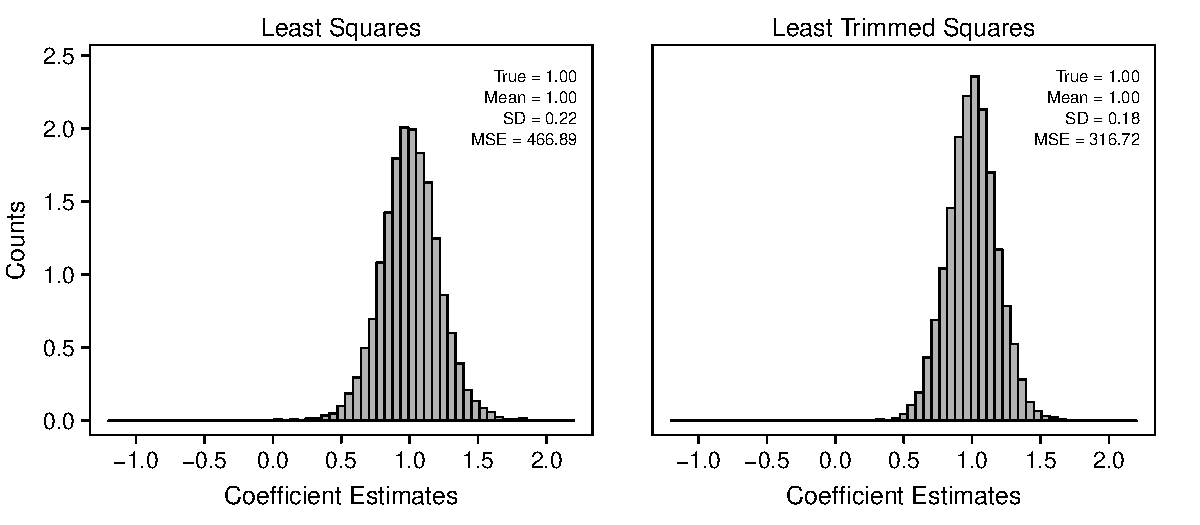
\includegraphics[scale = .7]{figs/lts-illustration.pdf}
\caption{Histograms of the sampling distribution for the least squares estimator and the least trimmed squares estimator under the true model $y = x + \epsilon$, where $\epsilon \sim t_3$. 
Note: despite least squares being the best linear unbiased estimator for the problem, the least trimmed squares estimator is a better estimator.}\label{fig:lts-illustration}
\end{center}
\end{figure}

But we also consider a least trimmed squares (LTS) estimator in which we minimize the smallest 90\% of the residuals. 
This method literally throws away data. 
Though it lacks the elegant theory of the least squares estimator, the right panel of Figure~\ref{fig:lts-illustration} shows that it is unbiased and more efficient that the least-squares estimator. 
The standard deviation of the estimates from the LTS estimator is about about 18\% smaller than the BLUE estimator, and the mean squared error is about 32\% smaller. 
By any reasonable standard, the LTS estimator is a better estimator than the least squares estimator in this example, yet the least squares estimator is BLUE\@. 
We obtain this improvement by expanding our focus to non-linear estimators, such as the LTS estimator. 
In this case, the LTS estimator is clearly non-linear because it places zero weight on the largest 10\% of the residuals and unit weight on the smallest 90\% of the residuals.

\section*{The Relative Emphasis on Standard Errors}

There has been much attention in the methodological literature to the sensitivity of standard errors to violations from the assumed model---and substantive scholars have paid attention.
White's (\citeyear{White1980}) seminal paper developing heteroskedasticity-consistent standard errors has received over 20,000 citations, making it one of the most cited papers in economics.
Beck and Katz's (\citeyear{BeckKatz1995}) development panel corrected standard errors has received over 4,300 citations, making it one of the most cited papers in political science.

On the other hand, there has been scant attention paid by substantive political scientists to the sensitivity of the \textit{estimates} to similar violations. 
This is particularly problematic, since it makes little sense to find a good standard error for a poor estimate (\citealt{Freedman2006} and \citealt{KingRoberts2014}). 
Two papers in political science have addressed the issue of robust estimation. 
\cite{Western1995} introduces political scientists to robust estimators, but this work has been essentially ignored. 
Although published in the same year \cite{BeckKatz1995}, \cite{Western1995} has received only 99 citations, or  about 2\% of the citations that Beck and Katz have received. 
Similarly, \cite{HardenDesmarais2011} have received only one citation, and it comes from the authors themselves.
Anderson's (\citeyear{Anderson2008}) broad and accessible introduction to robust estimation methods has received only about 150 citations, most from outside political science.

The relative focus on obtaining reasonable standard errors at the expense of reasonable estimates can be seen in Gujarati's (\citeyear{Gujarati2004}) popular econometrics text. Though the text deals with robust standard errors in some detail, \citet[p. 339]{Gujarati2004} writes in a footnote:
\begin{quote}
In passing, note that the effects of departure from normality and related topics are often discussed under the topic of robust estimation in the literature, a topic \textit{beyond the scope of this book} [italics ours].
\end{quote}
\cite{AngristPischke2009} devote an entire chapter to robust standard errors and completely ignore robust estimation of model coefficients. 
\cite{Wooldridge2013} does devote about two pages to robust estimation, though the tone is skeptical.

\section*{Dealing with Skewness: Transforming the Outcome}

Despite the lack of attention devoted by substantive scholars to non-normal errors,errors can deviate from normality in two ways and both negatively affect inferences when using least squares. 
\begin{enumerate}
\item The error distribution might be skewed. 
\item The error distribution might have heavy tails. 
\end{enumerate}

We suggest dealing with these two deviations differently, so we discuss each separately.

Skewed error distributions create two problems for the linear model. 
First, least squares estimates the quantity $E(y | X)$ and the mean is not a good summary of location for skewed variables. 
Symmetric error distributions are easier to understand. 

Second, and perhaps most importantly, skewed residuals from a least-squares fit indicate model misspecification. 
While we cannot be certain of the correct model in this situation, we can be confidence that the normal-linear model did not produce such data.
Sometimes, it is theoretically intuitive that explanatory variables have increasing effects on non-negative outcome variables, such as an individual's annual income. 
Rather than a college degree increasing one's expected income by \$10,000, perhaps a college degree increases it by 10\%. 
If this intuition is correct and a researcher relies on the statistical model $\text{Income}_i = \beta_0 + \beta_1 \text{College Degree}_i + \epsilon_i$, then the errors will have a strong skew to the right. Simply logging the outcome, or using the model $\log (\text{Income}_i) = \beta_0 + \beta_1 \text{College Degree}_i + \epsilon_i$, better captures the theoretical intuition.

Even if we remain indifferent toward the theoretical implications of skewed error distributions, we must remain cautious about the statistical implications. 
Indeed, the log-transformation in the example above improves the efficiency of the least squares estimator by making the assumption of normally-distributed errors more appropriate (not to mention the linearity of the model).
The performance of least squares estimators improves as the error distribution approaches a normal distribution. 

It is quite common in disciplines such as economics, for example, to log-transform non-negative outcome variables by default. 
Since non-negative (or strictly positive) outcomes are bounded below by zero, then these variables are likely skewed to the right---they are squeezed from the left by zero. 
In this case, the model $\log(y) = X\beta + \epsilon$ will likely provide a better approximation to the data.

When addressing skewed residuals, it is impossible to know whether (1) the skew is due to a misspecification of the outcome variable (i.e., failing to transform) or (2) the errors follow a heteroskedastic, skewed distribution. 
However, we can be confident that heavily skewed residuals are \underline{in}consistent with normal errors---the researcher must address the skew.
Transforming the outcome variable is \textit{one} effective method for making the model more consistent with the data.

\subsection*{The Box-Cox Transformation}

While we agree with the spirit of the suggestion to log-transform a non-negative outcome variable $y$, statisticians have created more precise empirical methods for choosing \textit{whether} and \textit{how} to do the transformation. 
\cite{BoxCox1964} propose the Box-Cox transformation 
\begin{equation}
   y^{(\lambda)} = BC(y, \lambda) =  \begin{cases}
    \dfrac{y^\lambda - 1}{\lambda} & \text{for } \lambda \neq 0\\
    \log y & \text{for } \lambda = 0
  \end{cases},
\end{equation}

\noindent where the transformation parameter $\lambda$ is estimated with maximum likelihood. 
In this case, the model becomes $y^{(\lambda)} = X\beta + \epsilon$. 
This is particularly convenient because $\hat{\lambda} \approx 1$ suggests no transformation is needed and $\hat{\lambda} \approx 0$ suggests that only an intuitive log-transformation is needed.

Researchers can easily assess the skewness in the residuals using a simple histogram of the residuals or a QQ plot of the residuals compared to their normal quantiles. 
For a formal test of skewness, researchers might use a direct test for symmetry on residuals $\hat{e}$, such as the Mira test \citep{Mira1999} or test whether $\lambda \neq 1$ under the Box-Cox framework. 
However, we do not want to argue for a particular test, but to highlight that (1) asymmetries worsen the performance of least squares and many robust methods, (2) researchers can easily detect asymmetries by carefully examining the residuals, and (3) researchers can address this problem with simple, easy-to-use transformations.

\subsection*{Mean or Median?}

Applying a non-linear transformation to the outcome variable $y$ does raise an interpretational difficulty. 
The usual, untransformed linear model is given by $y = X\beta + \epsilon$ and the quantity of interest is usually $E(y | X)$ or $\frac{\partial E(y | X)}{\partial x_j}$. 
For concreteness, consider the log-transformation. 
Using the same logic, then the model is $log(y) = X\beta + \epsilon$ and we might take the quantity of interest to be $E[\log(y) | X]$ or $\frac{\partial E[\log(y) | X]}{\partial x_j}$. 
However, the substantive researcher is usually interested in $y$, not $\log(y)$, making $\frac{\partial E[\log(y) | X]}{\partial x_j}$ more difficult to understand than $\frac{\partial E(y | X)}{\partial x_j}$. 
To make the results more interpretable, we need to ``undo'' the transformation. 
But $E[\log(y) | X] \neq \log [E(y | X)]$, which means that the log cannot be undone without additional computation.

These interpretational difficulties are not due to the choice to transform the data, but imbedded in the data themselves. 
The mean $E(\cdot)$ is not a good measure of the location of a skewed variable. 
While the mean often makes calculations easier, the median offers a better summary of location. 
The median also has an intuitive interpretation because one-half of the distribution lies above the median and one-half lies below. 
If a researcher uses $\med(y_{new} | X_{new})$ to predict the unknown outcome $y_{new}$ for a known case $X_{new}$, then she has a 50\% chance of being too high and a 50\% chance of being too low. 

In addition to the intuitive substantive interpretation of $\med(y | X)$, the median has another desirable property. 
Because the log-transformation is order-preserving, $\med[\log(y) | X] = \log [\med(y | X)]$, which means that the log \textit{can} easily be undone because $e^{\med[\log(y) | X]} = e^{\log[\med(y | X)]} = \med(y | X)$. 
Therefore, by adopting $\med(y | X)$ and $\frac{\partial \med(y | X)}{\partial x_j}$ as the quantities of interest, the researcher eases the interpretation of the results and can easily move between transformed and untransformed outcomes (e.g., $\med[\log(y)] \rightarrow \med(y)$). 
This holds for the more general case of $y^{(\lambda)}$ as well.

\subsection*{Simulating Quantities of Interest Under Transformation}

To obtain quantities of interest relating to $\med(y)$ when the estimated model has the generic form $y^{(\lambda)} = X\beta + \epsilon$, one can use the algorithm described by \cite{KingTomzWittenberg2000}.
\begin{enumerate}
\item Estimate the Box-Cox transformation parameter $\hat{\lambda}$ using maximum likelihood. 
(If the values one or zero fall within the confidence interval, then one may wish to use those values to maintain the direct interpretability of the model coefficients.)
\item Estimate the transformed model $y^{(\hat{\lambda})} = X\beta_{trans} + \epsilon$ and obtain the estimated model coefficients $\hat{\beta}_{trans}$ and covariance matrix $\Sigma_{trans}$.
\item Choose a hypothetical case or set of cases $X_{pred}$ for which to calculate the quantity of interest. 
If one is interested in calculating a first difference, it is convenient to use $X_{hi}$ and $X_{lo}$, where the first-difference $\Delta(y, X_{hi}, X_{lo}) = \med(y | X_{hi}) - \med(y | X_{lo})$.
\item Following \cite{KingTomzWittenberg2000}, for $i$ from one to a large (e.g., 1,000) number of iterations $n_{sims}$:
        \begin{enumerate}
        \item Simulate $\tilde{\beta}_{trans} \sim N\left(\hat{\beta}_{trans}, \Sigma_{trans}\right)$.
        \item If interested in the predicted value, then calculate and store $\tilde{Q}_i = \med(y | X_{pred}, \tilde{\beta}_{trans}) = BC^{-1}(X_{pred}\tilde{\beta}_{trans}, \hat{\lambda})$. If interested in the first-difference, the calculate and store $\tilde{Q}_i = \Delta(X_{hi}, X_{lo}, \tilde{\beta}_{trans}) = BC^{-1}(X_{hi}\tilde{\beta}_{trans}, \hat{\lambda}) - BC^{-1}(X_{lo}\tilde{\beta}_{trans}, \hat{\lambda})$.
        \end{enumerate}
\item Summarize the $n_{sims}$ simulations. 
The mean or median of $\tilde{Q}$ serves as an estimate of the quantity of interest and the standard deviation of $\tilde{Q}$ serves as an estimate of the standard error. The 5th and 95th percentiles of $\tilde{Q}$ serve as an estimate of the (likely asymmetric) 90\% confidence interval for the quantity of interest.
\end{enumerate}

\section*{Dealing with Heavy-Tails: $M$-Estimation}

In spite of the scant attention paid to robust estimators in political science, statisticians have developed and refined many robust methods since the seminal work of \cite{Box1953} and \cite{Huber1964}. 
\cite{HuberRonchetti2009} provide a detailed review of these developments and \cite{Anderson2008} provides an accessible introduction. 
Adjudicating among the many robust alternatives to least squares is beyond the scope of our paper, but, to fix ideas, we do introduce one robust estimator developed by \cite{BeatonTukey1974} in detail which has several desirable properties---the $M$-estimator with Tukey's biweight function. 
However, there are many other options: $M$-estimators with other objective functions (e.g., \citealt{Huber1973}), LMS- and LTS-estimators \citep{Rousseeuw1984}, S-estimators \citep{RousseeuwYohai1984}, and MM-estimators \citep{Yohai1987}.\footnote{User-friendly software to estimate models using these methods is available in both R and Stata. For the $M$-estimator with Tukey's biweight function, we particularly recommend the \texttt{rlm()} function in the R package \texttt{MASS} \citep{MASS} and the \texttt{rreg} command in Stata. For the other robust estimators, we point readers to the R package \texttt{robustbase} \citep{Rousseeuwetal2016} and the user command \texttt{robreg} in Stata \citep{Jann2010}.}

While least squares yields the coefficients that minimize the sum of the squared residuals, so that $\hat{\beta}^{ls} =\argmin_{b} \sum_{i = 1}^n (y_i - X_ib)^2$, M-estimators minimize an arbitrary, (usually) less-rapidly increasing function of the residuals $\hat{\beta}^{\rho} =\argmin_{b} \sum_{i = 1}^n \rho(y_i - X_ib)$. 
The function $\rho(\cdot)$ is typically chosen to be non-negative, symmetric about zero, and increasing away from zero. 
For example, \cite{HardenDesmarais2011} recommend the least absolute deviation (LAD) estimator \citep{Dodge1987} that such $\rho(\cdot) = \text{abs}(\cdot)$. 
However, other estimators offer better performance, particularly when the normal-linear model is approximately correct. 
In particular, we recommend Tukey's biweight function \citep{BeatonTukey1974}, so that

\begin{equation}
   \rho_{bw}(r_i) = \begin{cases}
     \dfrac{k^2}{6}\left\{ 1 - \left[ 1 - \left( \dfrac{r_i}{k} \right)^2 \right]^3\right\} & \text{for } |r_i| \leq k\\
        \dfrac{k^2}{6} & \text{for } |r_i| > k 
  \end{cases},
\end{equation}


\noindent where $r_i = y_i - X_ib$ and $k$ is a tuning parameter usually set to 4.685 to ensure good performance under the normal-linear model. 
We refer to the $M$-estimator using the biweight objective function as the ``biweight (BW) estimator.'' 
The BW estimator is a compelling alternative to the LAD estimator suggested by \cite{HardenDesmarais2011} for two reasons. 
First, the biweight objective function is redescending, which means that it has the ability to weight unusual observations all the way down to zero. 
The absolute value objective function, on the other hand, does downweight unusual observations, but these always received some weight. 
Secondly, the BW estimator is much more efficient than the LAD estimator when the errors are approximately normal. 

Two cautions are in order. 
First, the optimization problem is not convex, so standard minimization routines can produce a local rather than the global minimum. 
This concern might lead researchers to choose another objective function, such as the Huber objective function.
However, researchers can usually address this problem in practice by using a good starting value, such as the LTS estimate. 
Second, because the solution is not scale invariant, the residuals $\hat{e_i}$ are standardized by a robust estimate of scale $\hat{\sigma}_{mad}$, which must of course be estimated jointly, so that $\hat{\beta}^{bw} =\argmin_{b} \sum_{i = 1}^n \rho_{bw}\left(\dfrac{y_i - X_ib}{\hat{\sigma}_{mad}}\right)$, where $\hat{\sigma}_{mad} = \dfrac{\med\left( |y - Xb | \right)}{0.6745}$. 
Dividing by 0.6745 makes $\hat{\sigma}_{mad}$ a consistent estimator of the standard deviation of normal distribution.

While the theory for $M$-estimators remains less complete than the theory for least squares estimators, $M$-estimators do have desirable statistical properties. 
$M$-estimators are consistent as long as (1) $\rho(\cdot)$ is convex or (2) the errors follow strongly unimodal distribution (i.e., decreasing away from zero). 
Because the biweight objective function is not convex, we must assume that the errors follow a strongly unimodal distribution, which ensures that the estimates are consistent and distributed asymptotically normal.

$M$-estimators in general, and the biweight estimator in particular, have the desirable substantive property that they allow unusual cases to stand out.
Least squares, on the other hand, sacrifices fit on typical cases to better fit unusual cases. 
Allowing unusual cases to stand out, though, is extremely important because unusual cases can inform and improve subsequent analyses. 
Knowing what cases fall outside the explanatory power of the model enables the researcher to ask ``Why?'' and raise issues relating to concepts, theory, and measurement that might otherwise have been missed.

\subsection*{Estimation}

The model parameters $\hat{\beta}^{bw}$ and $\hat{\sigma}_{bw}$ can be quickly estimated jointly using the following iterative algorithm.
\begin{enumerate}
\item Start with initial estimate of the coefficients $\hat{\beta}^{(0)}$. The choice of initial estimator is not trivial. 
In the case of extreme outliers or many parameters, starting with least squares might lead the algorithm to a local minimum. 
We recommend using the least trimmed squares method discussed earlier to obtain starting values.
\item Extract the residuals $r^{(0)} = y - X\hat{\beta}^{(0)}$. 
Use these residuals to estimate the rescaled MAD so that $\hat{\sigma}^{(0)}_{mad} = \dfrac{\med\left( |r^{(0)}|\right)}{0.6745}$.
%\item Assign weights $w$ according to the function $\rho$ and denote $\text{diag}(w) = W$.
\item For $i$ from one until convergence:
        \begin{enumerate}
        \item Using $\hat{\beta}^{(i-1)}$ and $\hat{\sigma}^{(i-1)}_{mad}$ assign weights $w$ according to the function $\rho$ and denote $\text{diag}(w) = W^{(i)}$.
        \item Calculate $\hat{\beta}^{(i)} = (X'W^{(i)}X)^{-1}X'W^{(i)}y$.
        \item Calculate $\hat{\sigma}^{(i)}_{mad} = \dfrac{\med\left( |y - X\hat{\beta}^{(i)}|\right)}{0.6745}$
        \item The algorithm has converged when $r^{(i-1)} \approx r^{(i)}$.
        \end{enumerate}
\end{enumerate}

If we assume that the errors are symmetrically distributed about zero, then any objective function $\rho$ that is also symmetric about zero (including, for example, the biweight objective function) produces an unbiased estimate of the parameters. 
But this estimator is \textit{linear} if and only if $\rho(r_i) = r_i^2$. Other choices of $\rho(\cdot)$ might produce better estimators than the BLUE estimator.  

The theory for the variance for this broad class of unbiased $M$-estimators, though, is asymptotic. 
The required sample size for the asymptotic approximations to work well depends on the problem, but valid confidence intervals for small data can easily be computed by bootstrapping (\citealt{Efron1981} and \citealt{MooneyDuval1993}). 

\section*{Monte Carlo Simulations}

To understand and illustrate how the performance of the biweight (BW) estimator compares with the common least squares (LS) estimator, we conducted a Monte Carlo study. For comparison, we included the least trimmed squares estimator discussed above and the least absolute deviation (LAD) estimator suggested by \cite{HardenDesmarais2011}. To conduct the study, we simulated from the linear model $y = \beta_0 + \beta_1x_1 + \beta_2 x_2 + \beta_3 x_3 + \epsilon$, where $\beta_0 = 0$ and $\beta_1 = \beta_2 = \beta_3 = 1$ and the $x_i$'s were generated from independent standard normal distributions. 
We used six different distribution for the errors, each symmetric and centered at zero.
\begin{itemize}
\item \textit{Laplace distribution.} 
The Laplace distribution has tails that decrease exponentially, but behaves much differently from the normal distribution near zero. 
Rather than ``shoulders,'' the Laplace distribution has a sharp peak at zero and can be thought of as combining two exponential distributions, one in the positive direction and the other in the negative direction.
The LAD estimator is the maximum likelihood estimator when the errors follow a Laplace distribution.
\item \textit{$t_2$ distribution.} 
The $t$ distribution with two degrees of freedom has very heavy tails. 
Because the least squares estimator weights all points equally (conditional on $X$), the extreme outliers produced by the $t_2$ distribution makes least squares a very inefficient estimator.
\item \textit{$t_{10}$ distribution.} 
The $t$ distribution with ten degrees of freedom has \textit{slightly} heavier tails than the normal distribution. 
The $t_{10}$ and normal distributions are so similar that a Shapiro-Wilk test of normality only correctly rejects the null in about 65\% of repeated samples if 500 observation are simulated from a $t_{10}$ distribution.\footnote{One needs about 750 samples to reach 80\% power.} 
It is essentially impossible to spot the differences between the normal and $t_{10}$ density functions without plotting the two directly on top of each other.
\item \textit{Logistic distribution.} The logistic distribution has tails similar to the $t_{10}$ distribution---slightly heavier than the normal distribution. Researchers sometimes assume that latent errors in discrete choice models follow a logistic distribution \citep{Train2009}.
\item \textit{Uniform distribution.} Simply for comparison, we include a uniform distribution from -1 to 1.
\item \textit{Normal Distribution.} The normal distribution yields the optimal conditions for the LS estimator. 
When the errors follow a normal distribution, the LS estimator has the smallest variance of all unbiased estimators. 
\end{itemize}

For the six different error distributions, we simulated 10,000 data sets with 100 observations each and estimated $\beta_1$ using the LS estimator, the BW estimator, the LAD estimator, and the LTS estimator. 
For each condition, we calculated the mean squared error (MSE) of the estimate of $\beta_1$. 
To simplify the presentation, we divided the MSE of the BW, LAD, and LTS estimators by the MSE of the LS estimator. 
Table~\ref{tab:mc-sims-100} provides the results. 
These results show that the MSE varies considerably across the estimators for each error distribution.

\begin{table}[h!]
{\scriptsize
% quantreg::latex.table(x = ta, file = "doc/tabs/mc-sims-100",      rowlabel = "", cgroup = c("Mean", "Standard Deviation", "Mean Squared Error"),      rgroup = c("Absolute Performance", "Relative Performance"),      n.rgroup = c(3, 2), dec = 3, table.env = FALSE, label = "tab:mc-sims-100") 
%
\begin{center}
\begin{tabular}{|l||c|c|c|c||c|c|c|c||c|c|c|c|} \hline
\multicolumn{1}{|l||}{\bf }&\multicolumn{4}{c||}{\bf Mean}&\multicolumn{4}{c||}{\bf Standard Deviation}&\multicolumn{4}{c|}{\bf Mean Squared Error}\\ \cline{2-13}
\multicolumn{1}{|l||}{}&\multicolumn{1}{c|}{Lapl.}&\multicolumn{1}{c|}{$t_2$}&\multicolumn{1}{c|}{$t_{10}$}&\multicolumn{1}{c||}{Norm.}&\multicolumn{1}{c|}{Lapl.}&\multicolumn{1}{c|}{$t_2$}&\multicolumn{1}{c|}{$t_{10}$}&\multicolumn{1}{c||}{Norm.}&\multicolumn{1}{c|}{Lapl.}&\multicolumn{1}{c|}{$t_2$}&\multicolumn{1}{c|}{$t_{10}$}&\multicolumn{1}{c|}{Norm.}\\ \hline
{\bf Absolute Performance}&&&&&&&&&&&&\\
~~Least Squares&~~~0.999&~~~1.000&~~~1.001&~~~0.999&~~~0.151&~~~0.319&~~~0.114&~~~0.099&~227.419&1016.182&~130.867&~~98.850\\ 
~~Least Absolute Deviation&~~~0.999&~~~0.999&~~~1.003&~~~1.000&~~~0.126&~~~0.146&~~~0.131&~~~0.124&~159.499&~212.360&~172.911&~154.714\\ 
~~Tukey's Biweight&~~~1.000&~~~0.999&~~~1.001&~~~0.999&~~~0.131&~~~0.138&~~~0.113&~~~0.102&~172.043&~189.519&~127.731&~104.759\\ \hline
{\bf Relative Performance}&&&&&&&&&&&&\\
~~LAD/LS&~~~1.001&~~~0.999&~~~1.002&~~~1.001&~~~0.837&~~~0.457&~~~1.149&~~~1.251&~~~0.701&~~~0.209&~~~1.321&~~~1.565\\ 
~~BW/LS&~~~1.001&~~~1.000&~~~1.000&~~~1.000&~~~0.870&~~~0.432&~~~0.988&~~~1.029&~~~0.757&~~~0.187&~~~0.976&~~~1.060\\ 
\hline
\end{tabular}
\end{center}

}
\caption{The MSE of the BW, LAD, and LTS estimators compared to the LS estimator for six different error distributions with a sample size of 100. \\
Note: the BW has the best or nearly best performance in each condition, while the LAD and LTS estimators performs quite poorly for the $t_{10}$ and normal distributions and the LS estimator performs quite poorly for the Laplace and $t_2$ distributions.}\label{tab:mc-sims-100}
\end{table}

The LAD estimator is the MLE when the errors follow a Laplace distribution, so, as we might expect, the LAD performs well for Laplace errors, with a MSE about 30\% lower than the LS estimate. 
However, the BW estimator also performs quite well for the Laplace distribution, with a MSE about 25\% less than the LS estimator. The LTS estimator performs the worst of the robust estimators, but the MSE of the LTS estimator is still about 5\% less than the MSE for the LS estimator.

The $t_2$ distribution is nearly a worst case for the LS estimator, so all three robust alternatives perform considerably better. 
The BW estimator has an MSE about 85\% lower than the LS estimator and the LAD and LTS estimators have a MSE about 83\% and 82\% lower, respectively. 

The $t_{10}$ distribution is a much more interesting case, because it is very similar to a normal distribution. 
Indeed, even statistical tests have trouble distinguishing the $t_{10}$ from the normal, even with large samples (e.g., with $N = 500$, the Shapiro-Wilk test of normality has about 65\% power). 
In this case, the LAD and LTS estimators have a 33\% and 44\% larger MSE than the LS estimator, respectively.
The BW estimator, on the other hand, shows a small \textit{improvement} over the LS estimator, with an MSE about 2\% \textit{smaller} than the LS estimator. 
This is crucial because it shows that only a small deviation from normality is required before the BLUE estimator is no longer a BUE estimator. 

The logistic and $t_{10}$ distributions are similar and produce similar results. The LAD and LTS estimators perform worse than the LS estimator, with the MSE 24\% and 31\% larger than the LS estimator, respectively. Again, though, the BW estimator shows a small improvement over the LS estimator, with an MSE about 5\% smaller than the LS estimator. 

For the uniform distribution, the LAD and LTS estimators perform much worse than the LS estimator, with an MSE 171\% and 288\% larger, respectively. However, the BW estimator performs similarly to the LS estimator with an MSE only 16\% larger.

The normal distribution is the optimal scenario for the LS estimator and it outperforms the LAD and LTS estimator considerably when the errors are normal. 
In this situation, the MSE for the LAD and LTS estimator is 58\% and 71\% larger than the MSE for the LS estimator, respectively. 
However, the BW estimator performs nearly as well as the LS estimator for normal errors. 
The MSE for the BW estimator is only about 6\% larger than the MSE for the LS estimator.

Among the estimators we consider, the BW estimator does not have the smallest variance for the Laplace, uniform, or normal distributions, but it is a \textit{close} second. 
It does have the smallest variance for the $t_2$, $t_{10}$, and logistic distributions. 
It considerably outperforms the LS estimator for Laplace and $t_2$ errors and the LAD and LTS estimators for normal and $t_{10}$, logistic, and uniform errors. 
Thus, the BW estimator works quite well across a range of error distributions, whereas the LS, LAD, and LTS estimators work well only in particular situations. 
And even in particular situations where the LS, LAD, and LTS estimators work well, the BW estimator performs comparably.

To better understand how the heaviness of the tails of the error distribution affects the efficiency of these estimators, we repeated these simulates for $t$ distributions with degrees of freedom ranging from two to thirty and sample sizes 25, 100, 500, and 2,000. Figure~\ref{fig:mc-sims} shows the MSE of the LAD and BW estimators relative to the LS estimator.

\begin{figure}[h!]
\begin{center}
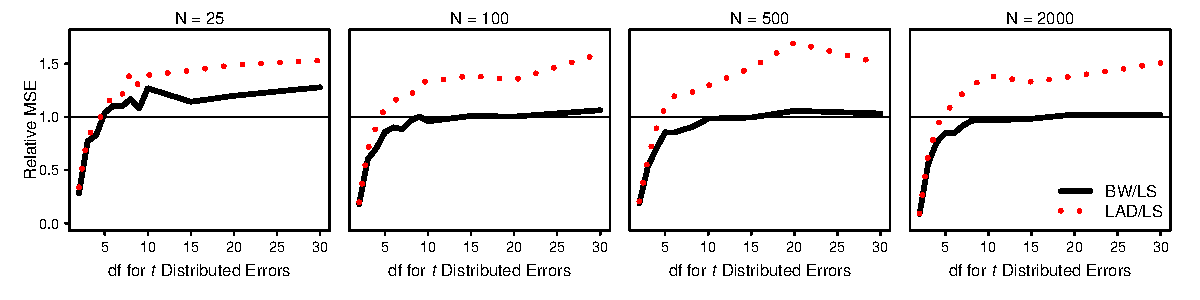
\includegraphics[width = \textwidth]{figs/mc-sims.pdf}
\caption{The relative MSE for the BW, LAD, and LTS estimators compared to the LS estimator for $t$ distributed errors as the degrees of freedom varies. \\
Note: for very heavy-tailed distributions (e.g., two to five degrees of freedom), the BW, LAD, and LTS estimators significantly outperform the LS estimator. 
And while the performance of the LAD and LTS estimators significantly worsens as the distribution becomes more normal, the BW estimator remains comparable to the LS estimator.}\label{fig:mc-sims}
\end{center}
\end{figure}

Notice that the BW, LAD, and LTS estimators perform quite well for very heavy-tailed distributions (i.e., degrees of freedom from two to four), but as the tails grow lighter, the LS estimator quickly begins to outperform the LAD and LTS estimator. 
Except for all but very heavy-tailed distributions, the LS estimator is considerably more efficient than the LAD and LTS estimators. 

The BW estimator, other the other hand, is a much stronger competitor for the LS estimator. 
While the LS estimator is more efficient for lighter-tailed distributions (i.e., more than ten degrees of freedom), the difference is tiny except in very small samples. 
Indeed, for sample sizes of 100 or larger, the LS estimator is only about 5\% more efficient than the BW estimator \textit{at best}. 
This second simulation also suggests that the BW estimator works almost as well as the LS estimator under ideal conditions for LS estimator and considerably better across a wide range of other, substantively plausible scenarios.

\section*{Recommendation for Applied Researchers}

When using the linear model, we suggest that researchers take steps to ensure that the assumption of normal errors makes theoretical and empirical sense. 
\begin{enumerate}
	\item Initially fit the model using least squares. 
	\item As a ``robustness check,'' re-fit the model using a robust alternative, such as the biweight estimator. 
	\item If the inferences change (and even if not), carefully examine the residuals using histograms and QQ plots. Be careful to check for skewness.
	\item If the residuals are not symmetrically distributed, then consider a transformation. 
	This transformation might be critical because it allows the model to represent non-linear relationships implied by the skewness and allows the statistical model to more closely approximate the data. 
	The log-transformation has a nice substantive interpretation, so it makes sense as a first cut, especially for variables naturally bounded below by zero or one. 
	If the log-transformation over- or under-corrects the skewness, then the Box-Cox transformation should ensure that the residuals are roughly symmetric.
	\item Once the residuals are roughly symmetric, it makes sense to re-fit the model using least squares and a robust alternative. 
	Especially if the residuals appear to have heavy tails, then the robust estimator might serve as a more efficient estimator. 
	However, the robust estimator also allows for greater substantive interpretation as well, because it allows unusual cases to stand out.
	\item Always pay close attention to the residuals from each model, especially differences, as these can be especially substantively informative.
	\item To the extent that some cases seem unusual, especially with robust regression, give these cases careful review. 
	Is it possible that these unusual outcomes are  data entry errors? 
	In light of these cases, can the measurement be improved? 
	Might a subset of the cases be operating under a substantially different causal process that could be built into the statistical model? 
\end{enumerate}

To illustrate these recommendations, we include a reanalysis of \cite{ClarkGolder2006} as an online appendix. 

\section*{Conclusion}

In our paper, we adopt and defend a skeptical perspective toward least squares and explain the importance of carefully scrutinizing residuals.
We first observe that the restriction to linear estimators, as required by the Gauss-Markov theorem, is unnecessary, artificial, and counterproductive. 
When the errors do not follow a normal distribution, restricting ourselves to linear estimators limits our ability to efficiently estimate the model coefficients. And as \cite{BerryFeldman1985} claim, the assumption of normal errors is usually difficult to defend using either theory or data. 

Secondly, we use Monte Carlo simulations to show that our preferred estimator, an $M$-estimator with a biweight objective function, performs almost as well as least squares for normal errors, slightly better than least squares for small deviations from normality, and much better than least squares for large deviations from normality. 
In our view, political scientists should prefer this robust behavior to the more fragile least squares estimator.

Thirdly, we use a practical example to show that a more robust estimator can \textit{constructively} alter substantive conclusions. 
Robust estimators not only estimate the model coefficients more efficiently under deviations from normality, but more importantly, allow unusual cases to stand out as unusual. 
This, in turn, allows researchers to identify and carefully investigate these cases and improve the theoretical model, the statistical model specification, and the measurement of the concepts.

\singlespace
\bibliographystyle{apsr_fs}
\bibliography{bibliography.bib}

\end{document}
